% Learn Latex: https://www.overleaf.com/learn/latex/Learn_LaTeX_in_30_minutes

\documentclass[12pt]{article}
\usepackage[utf8]{inputenc}
\usepackage[english]{babel}
\usepackage{indentfirst}
\usepackage{graphicx}
\usepackage{caption}
\usepackage{float}
\usepackage[margin=1.2in]{geometry} % margins
\usepackage{multicol}
\usepackage{wrapfig}
\usepackage{amsmath}
\usepackage{amssymb}
\usepackage[colorlinks=true, linkcolor=blue, urlcolor=cyan]{hyperref}

\graphicspath{{./Figures/}}
\setlength{\parskip}{1em} % paragraph spacing
\renewcommand{\baselinestretch}{1.5} % line spacing
\addto\captionsenglish{\renewcommand{\contentsname}{Units}} % Change TOC title

\title{\textbf{AP Calculus BC:\\Notes, Formulas,  Equations,\\and Examples}}
\author{Bryan Deng}
\date{Start date: March 2, 2021\\Last updated: \today}

\begin{document}
    \maketitle
    \vfill
    \centering \textit{Sections based off of
        \href{https://www.khanacademy.org/math/ap-calculus-bc}{Khan Academy} units.
        \\ Formatting may not be the best, this is just a study tool. (Still a work in progress.)}
        \\ \textcopyright 2021 Bryan Deng
    \newpage

    % table of contents followed by horizontal line
    \raggedright
    \tableofcontents
    \par\noindent\rule{\textwidth}{0.4pt} % horizontal line
    \newpage

    \addcontentsline{toc}{section}{Introduction}
    \section*{Introduction}
        The percentages beside the section titles are how much of the AP Calculus BC exam score will be of that topic. (Percentages based off of College Board website.)
        \newline \newline
        \textbf{Resources:}
        \begin{itemize}
            \item \href{https://apstudents.collegeboard.org/courses/ap-calculus-bc}{College Board Website}
            \item \href{https://www.khanacademy.org/math/ap-calculus-bc}{Khan Academy}
            \item \href{https://www.math24.net/topics-calculus}{Math 24 (Quick explanations of topics)}
            \item \href{https://www.math.ucdavis.edu/~kouba/CalcOneDIRECTORY/}{Practice Questions + Solutions}
            \item \href{https://www.chelmsford.k12.ma.us/site/handlers/filedownload.ashx?moduleinstanceid=2496&dataid=7289&FileName=AP%20Calculus%20BC%20Syllabus.pdf}{BC Exam Syllabus (Not the most organized but good enough)}
        \end{itemize}
        I have tried my best to provide links to all sources.

    \raggedright
    \section{Limits and Continuity (4\% - 7\%)}
    \par\noindent\rule{\textwidth}{0.1pt}
        The limit is when a given value approaches, or gets \textit{really close} (infinitely) to another value. The standard notation for a limit:
        \[ \lim_{x \to c} f(x) \]
        when $x$ can approach $c$ from either the left ($-$) or the right ($+$). By adding a sign superscript to the $c$, it means the $x$ can only approach from that direction:
        \[ \lim_{x \to c^+} f(x) \]
        \centering{
        \textit{Right hand limit}, $x$ approaches $c$
        from values greater than $c$.
        \[ \lim_{x \to c^-} f(x) \]
        \textit{Left hand limit}, $x$ approaches $c$
        from values greater than $c$.
        }

        \raggedright
        \subsection{Limits to Infinity}
            If a degree (biggest exponent) of a polynomial is greater than or equal to $1$, its limit as $x$ approaches $\pm\infty$ will also be $\pm\infty$. This depends on the sign of the leading coefficient and the degree of the polynomial.
            \\ Example:
            \begin{align*}
                &f(x) = 3x^3 - 7x^2 + 2 \\
                \lim_{x \to \infty} &f(x) = \infty \\
                \lim_{x \to -\infty} &f(x) = -\infty
            \end{align*}
            The degree of $f(x)$ is $3$, and the leading coefficient it positive. The graph goes down to up from left to right.
            \newline \newline
            With Fractions, just find whether the highest degree is in the numerator or the denominator. Numerator means $\infty$, denominator means $0$.

            \subsection{Asymptotes}
            \begin{wrapfigure}[11]{r}{0.5\textwidth}
                \begin{center}
                    \frame{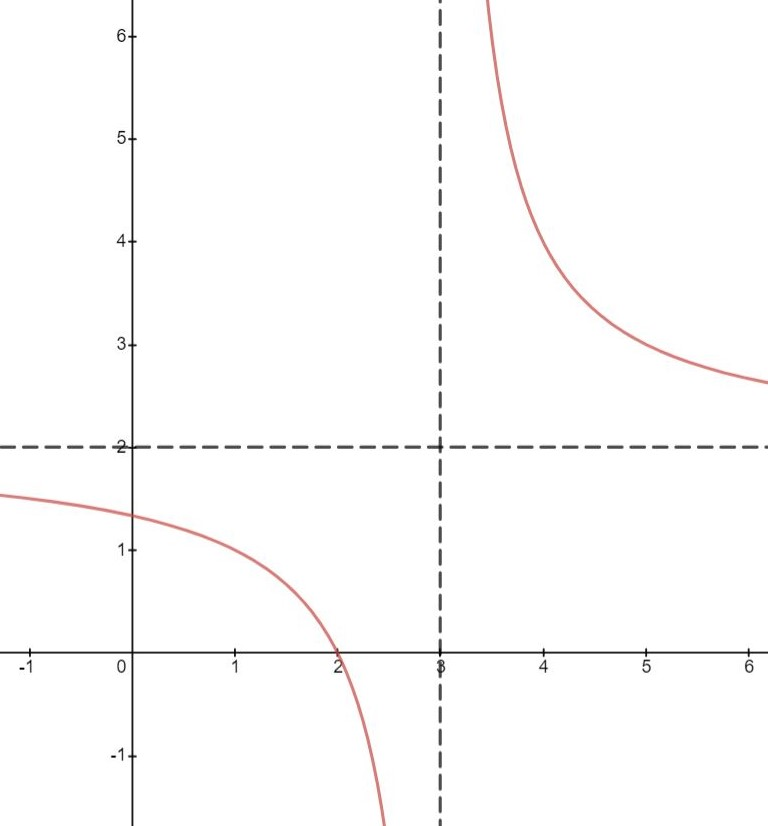
\includegraphics[scale=0.4]{fig1.JPG}}
                \end{center}
                \caption{$f(x) = \frac{2x-4}{x-3}$}
            \end{wrapfigure}

            Sometimes functions can have asymptotes, either vertical or horizontal. In the case of vertical asymptotes, the limit would be \textit{unbounded} as it approaches that $x$ value.
            \\ Example (Figure 1):
            \begin{align*}
                &f(x) = \frac{2x-4}{x-3} \\
                \lim_{x \to 3} &f(x) = \text{undef} \\
                \lim_{x \to 3^-} &f(x) = -\infty \\
                \lim_{x \to 3^+} &f(x) = \infty
            \end{align*}

            As with horizontal asymptotes, as $x$ approaches $\pm \infty$, the limit would actually approach the horizontal asymptote. Although the $y$-value never actually touches the asymptote, the limit gets really close to the value, from both below and above.
            \\ Example: (also Figure 1):
            \begin{align*}
                &f(x) = \frac{2x-4}{x-3} \\
                \lim_{x \to \infty} &f(x) = 2 \\
                \lim_{x \to -\infty} &f(x) = 2
            \end{align*}

        \subsection{Limit Properties}
            The limits of combined functions can be found by finding the limit of each of the individual functions, then applying the operations. All the following examples will be based on Figure 2.
            \begin{figure}[H]
                \begin{center}
                    \frame{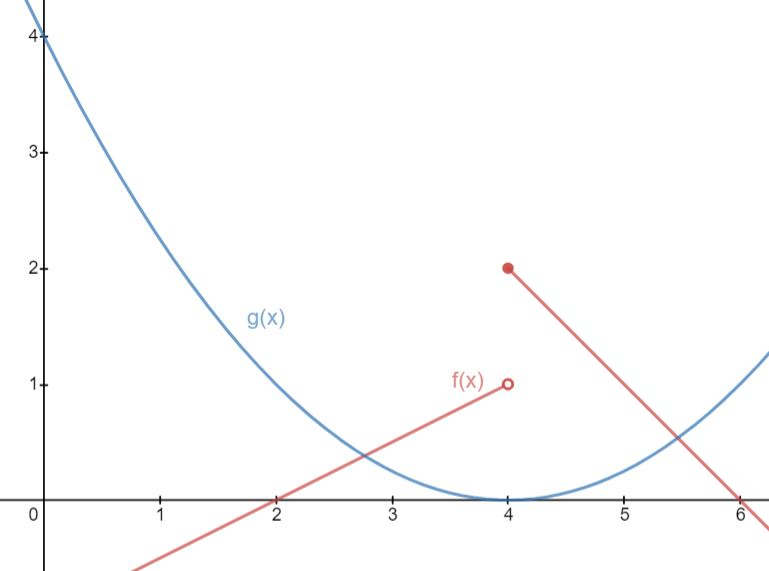
\includegraphics[scale=0.5]{fig2.JPG}}
                    \caption[Figure 2]{}
                \end{center}
            \end{figure}
            \begin{itemize}
                \item \textbf{Addition/Subtraction:}
                    \newline
                    When taking the limit of the sum or difference of multiple functions, it's the same thing as taking the sum or difference of each of the separate limits or each function.
                    \newline
                    \noindent\begin{minipage}{0.5\linewidth}
                        \begin{align*}
                            &\lim_{x \to 2} \left[ f(x) + g(x) \right] \\
                            &= \lim_{x \to 2} f(x) + \lim_{x \to 2} g(x) \\
                            &= 0 + 1 \\
                            &= 1
                        \end{align*}
                    \end{minipage}%
                    \begin{minipage}{0.5\linewidth}
                        \begin{align*}
                            &\lim_{x \to 2} \left[ g(x) - f(x) \right] \\
                            &= \lim_{x \to 2} g(x) - \lim_{x \to 2} f(x) \\
                            &= 1 - 0 \\
                            &= 1
                        \end{align*}
                    \end{minipage}
                    \newline
                    \begin{align*}
                        &\lim_{x \to 4} \left[ f(x) + g(x) \right] \\
                        &= \lim_{x \to 4} f(x) + \lim_{x \to 4} g(x) \\
                        &= \text{undef} + 0 \\
                        &= \text{undef}
                    \end{align*}

                    Note that in the above equation, because the right and left side limits of $f(x)$ are not the same, its limit is \textit{undefined}. If just one of the functions has an undefined limit, the combined limit would also be undefined.
                    \\ \textbf{The extended Sum Rule:}
                    \begin{equation*}
                        \lim_{x \to c} \left[ f_1(x) + \cdots + f_n(x) \right]
                        = \lim_{x \to c} f_1(x) + \cdots + \lim_{x \to c} f_n(x).
                    \end{equation*}
                    \newline

                \item \textbf{Multiplication:}
                    \newline
                    Multiplication of the limits of functions is quite straightforward.
                    \begin{align*}
                        &\lim_{x \to 2} \left[ f(x) \cdot g(x) \right] \\
                        &= \lim_{x \to 2} f(x) \cdot \lim_{x \to 2} g(x) \\
                        &= 0 \cdot 2 \\
                        &= 0
                    \end{align*}
                    \newline
                    The same exception applies when one of the limits is \textit{undefined}. This just makes the entire combined limit undefined.
                    \\ \textbf{The extended Product Rule:}
                    \begin{equation*}
                        \lim_{x \to c} \left[ f_1(x) f_2(x) \cdots f_n(x) \right]
                        = \lim_{x \to c} f_1(x) \cdot \lim_{x \to c} f_2(x)
                        \cdots f_n(x).
                    \end{equation*}
                    \newline

                \item \textbf{Division:}
                    \newline
                    Division is once again basically the same as the other basic operations. There's only one exception, when the denominator is $0$.
                        \begin{align*}
                            &\lim_{x \to 2} \frac{g(x)}{f(x)} \\
                            &= \frac{\lim_{x \to 2} g(x)}{\lim_{x \to 2} f(x)} \\
                            &= \frac{1}{0} \\
                            &= \text{undef}
                        \end{align*}
                    \\ \textbf{General quotient rule:}
                    \begin{equation*}
                        \lim_{x \to c} \frac{f(x)}{g(x)}
                        = \frac{\lim_{x \to c} f(x)}{\lim_{x \to c} g(x)},
                        \quad \textrm{iff} \quad \lim_{x \to c} g(x) \ne 0
                    \end{equation*}
                    \newline

                \item \textbf{Composite Functions:}
                    \newline
                    When working with limits of composite functions, it's the same thing as taking the limit of the inner function, then just evaluating the outer function normally.
                    \begin{align*}
                        &\lim_{x \to 1} f\left(g(x)\right) \\
                        &= f\left( \lim_{x \to 1} g(x) \right) \\
                        &= f(2) \\
                        &= 0
                    \end{align*}
                    \newline
                    If the limit of the inner function is undefined, the entire equation would also be undefined.
                    \newline
                    \begin{align*}
                        &\lim_{x \to 4} g\left( f(x) \right) \\
                        &= g\left( \lim_{x \to 4} f(x) \right) \\
                        &= g(\text{undef}) \\
                        &= \text{undef}
                    \end{align*}
                \item \textbf{Other Theorems:}
                    \newline
                    Given that $\lim f(x)$ and $\lim g(x)$ are both finite
                    for all numbers, and $C$ is a constant:
                    \newline
                    \noindent \begin{minipage}{0.5\linewidth}
                        \[ \lim k f(x) = k \lim f(x) \]
                    \end{minipage}%
                    \begin{minipage}{0.5\linewidth}
                        \[ \lim_{x \to a} C = C \]
                    \end{minipage}
            \end{itemize}

        \subsection{Solving Limits}
            The first thing to always try when solving limits is \textbf{direct substitution}.
            If this does not work (undefined limit, 0 as denominator, etc.), then algebraic manipulation (factoring) is the next step.
            \newline
            \begin{align*}
                &\lim_{x \to 2} \frac{x^4 + 3x^3 - 10x^2}{x^2 - 2x} \\[6pt]
                &= \lim_{x \to 2} \frac{x^2\left[ (x+5)(x-2) \right]}{x(x-2)} \\
                &= \lim_{x \to 2} x(x+5) \\
                &= 14
            \end{align*}
            \newline
            When encountering radicals, conjugates can be used.
            \newline
            \begin{align*}
                &\lim_{x \to -4} \frac{x+4}{\sqrt{3x+13}-1} \\[6pt]
                &= \lim_{x \to -4} \frac{x+4}{\sqrt{3x+13}-1} \cdot \frac{\sqrt{3x+13}+1}{\sqrt{3x+13}+1} \\[6pt]
                &= \lim_{x \to -4} \frac{(\sqrt{3x+13}+1)(\sqrt{3x+13}+1)}{3x+13-1} \\[6pt]
                &= \lim_{x \to -4} \frac{(x+4)(\sqrt{3x+13}+1)}{3(x+4)} \\[6pt]
                &= \lim_{x \to -4} \frac{\sqrt{3x+13}+1}{3} \\[6pt]
                &= \frac{2}{3}
            \end{align*}
            \newline
            When dealing with trigonometric equations, use trig identities (if direct substitution does not work).
            \newline
            \begin{align*}
                &\lim_{x \to \frac{\pi}{2}} \frac{\cot^2(x)}{1-\sin(x)} \\[6pt]
                &= \lim_{x \to \frac{\pi}{2}} \frac{\cos^2(x)}{\left( \sin^2(x) \right)\left(1-\sin(x)\right)} \\[6pt]
                &= \lim_{x \to \frac{\pi}{2}} \frac{1-\sin^2(x)}{\left( \sin^2(x) \right)\left(1-\sin(x)\right)} \quad \text{(Pythagorean's Identity)} \\[6pt]
                &= \lim_{x \to \frac{\pi}{2}} \frac{\left( 1+\sin(x) \right)\left( 1-\sin(x) \right)}{\left( \sin(x) \right)\left(1-\sin(x)\right)} \\[6pt]
                &= \lim_{x \to \frac{\pi}{2}} \frac{1+\sin(x)}{\sin^2(x)} \text{, for } x \ne (2k+1)\frac{\pi}{2}\\[6pt]
                &= 2
            \end{align*}
            \newline
            However, functions can not always be factored, so in that case they will just be undefined.
            \newline
            \begin{align*}
                &\lim_{x \to 1} \frac{2x}{x^2 - 7x + 6} \\[6pt]
                &= \lim_{x \to 1} \frac{2x}{(x-6)(x-1)} \\
                &= \frac{2}{0} \\
                &= \text{undef}
            \end{align*}
            \newline
            The different results achievable from direct substitution can mean different things. $\frac{k}{0}$ means that the limit does not exist, probably an asymptote. $\frac{0}{0}$ means that the limit is indeterminate, use manipulation and try again.

        \subsection{Continuity}
            A function is continuous at a point if its right and left hand side limits at that point are the same. In other words, it ``can be drawn without lifting the pencil.''
            \[ \lim_{x \to c^-} f(x) = \lim_{x \to c^+} f(x).\]
            For a function to be \textit{continuous for all real numbers}, it has to give a real number result for all real number $x$. Basically it's continuous
            over its \textbf{domain} (horizontal).
            \begin{itemize}
                \item $\sqrt{x+4}$ is continuous for all $x \ge -4$.
                \item $\sqrt[5]{x}$ is continuous for all $x \in \mathbb{R}$ (odd roots can handle negatives).
                \item $\ln{x}$ is continuous for all $x \ge 0$.
                \item $\frac{1}{x-3}$ is continuous for $x \ne 3$.
            \end{itemize}
            \textbf{Removable discontinuity} is a function, where the point of discontinuity can be ``removed,'' and the graph of the new function would be almost identical to the original function.
            \\ Given:
            \[ \lim_{x \to c} f(x) = k < \infty, \]
            where:
            \[ F(x) = \begin{cases}
                f(x) &\text{for } x \ne c \\
                k &\text{for } x = c,
            \end{cases} \]
            then $F(x)$ has removable discontinuity at $k$.
            \newline
            \textbf{Jump discontinuity} is when a part of a graph jumps from one $y$ to another on the same $x$ value. % too lazy to insert example
            \newline
            \textbf{Infinite discontinuity} is basically where there is a vertical asymptote.

        \subsection{Squeeze Theorem}
            When it is hard to find the limit for a function, the squeeze theorem (AKA sandwich theorem) can be used. Basically find two other functions, one on top, and one below, and use the limits of the two functions to ``squeeze'' the limit of the given function.
            \\ Given
            \[ f(x) \le g(x) \le h(x) \]
            for all $x$ in an open interval that includes $c$, and
            \[ \lim_{x \to c} f(x) = \lim_{x \to c} h(x) = L, \]
            then,
            \[ \lim_{x \to c} g(x) = L. \]
            Note that $x$ and $L$ can both be $\pm \infty$.
            \newline
            \\ Example:
            \begin{align*}
                &\text{Problem:} &&\lim_{x \to \infty} \frac{\sin{x}}{x} \\[6pt]
                &\text{keep in mind that} &-1 &\le \sin{x} \le 1 \\
                &\text{divide by $x$} &\frac{-1}{x} &\le \frac{\sin{x}}{x} \le \frac{1}{x} \\[6pt]
                &\text{take limits of smaller functions } &\lim_{x \to \infty} \frac{-1}{x} &= 0 = \lim_{x \to \infty} \frac{1}{x} \\[6pt]
                &\text{Squeeze Theorem:} &\lim_{x \to \infty} &\frac{\sin{x}}{x} = 0.
            \end{align*}
            The best way to solve the above problem is to first recognize the easier part of the problem, $\sin{x}$. Then manipulate the entire inequality so the middle function becomes the original problem. Solve limits of the two other functions to solve original limit.
            \\ Another example:
            \begin{gather*}
                \lim_{x \to -\infty} \frac{x^2(\sin{x} + \cos^{3}{x})}{(x^2+1)(x-3)} \\[8pt]
                \text{Note that:} \\
                -1 \le \sin{x} \le 1, \\
                \because -1 \le \cos{x} \le {1} \\
                \therefore -1 \le \cos^{3}{x} \le 1 \\
                -2 \le \sin{x} + \cos^{3}{x} \le 2 \\[8pt]
                \text{$x$ is approaching negative $\infty$, so $(x-3) < 0$} \\
                \frac{-2}{x-3} \ge \sin{x} + \cos^{3}{x} \ge \frac{2}{x-3} \\[6pt]
                \frac{2x^2}{(x^2+1)(x-3)} \ge \sin{x} + \cos^{3}{x} \ge \frac{-2x^2}{(x^2+1)(x-3)} \\[10pt]
                \lim_{x \to -\infty}\frac{2x^2}{(x^2+1)(x-3)} = 0 \\[6pt]
                \lim_{x \to -\infty}\frac{-2x^2}{(x^2+1)(x-3)} = 0 \\[6pt]
                \therefore \quad \lim_{x \to -\infty} \frac{x^2(\sin{x} + \cos^{3}{x})}{(x^2+1)(x-3)} = 0
            \end{gather*}

        \subsection{Intermediate Value Theorem} % whats this?
            Given a \textbf{continuous} segment of a function $f(x)$, let $c \in [a, b]$ and $w$ be in between $f(a)$ and $f(b)$. Then there must be \textbf{at least} on value $c$ such that $f(c) = w$. In short, a continuous line from $a \to b$ must pass through every $x$ and $y$ value in between them. (Refer to \hyperref[fig:intvaltheorem]{Figure 3}.)
            \newline
            \\ This goes both ways. If there is a $c$, then there is  $w$. If there is a $w$, then there is $c$.
            \begin{figure}[H]
                \begin{center}
                    \frame{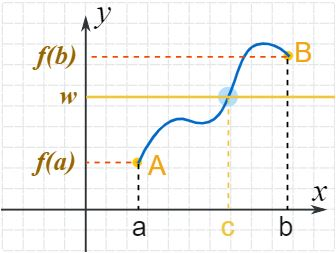
\includegraphics[scale=0.8]{fig3.JPG}}
                    \caption{\href{https://www.mathsisfun.com/algebra/intermediate-value-theorem.html}{source}}
                    \label{fig:intvaltheorem}
                \end{center}
            \end{figure}

    \section{Differentiation: Definition and Fundamental Properties (4\% - 7\%)}
    \par\noindent\rule{\textwidth}{0.1pt}
        A derivative is the \textbf{instantaneous} rate of change of a function at a point. It's the average rate of change over an infinitely small interval. It has two main notations (names are not important here).
        \begin{itemize} % too lazy to keep notation usage uniform across document
            \item \textbf{Lagrange's notation}:
            The derivative of $f(x)$ is $f'(x)$, pronounced ``f prime''. Higher order derivatives are written like $f''(x)$ or $f^2(x)$. In general it's written as $f^{n}(x)$, or with $n$ ticks.
            \item \textbf{Leibniz's notation}:
            The derivative of $f$ is $\frac{d}{dx}$, indicating a derivative with respect to $x$. When $y=f(x)$ the derivative can be written as $\frac{dy}{dx}$. Higher order derivatives are written like $\frac{d^{n}y}{dx^{n}}$.
        \end{itemize}

        \subsection{Continuity and Differentiability}
            \textbf{Differentiability}: the function must be differentiable for every value in its domain.
            \\ \textbf{Continuity}: the function has no breaks over its domain, ``can be drawn without lifting the pencil.''
            \newline
            Differentiability \textit{implies} continuity, but continuity does not mean differentiability.

        \subsection{Derivative as a Limit}
            Not the most useful, but might be on exam. College Board says: ``You'll apply limits to define the derivative.''
            \[ \frac{d}{dx} f(x) = \lim_{h \to 0} \frac{f(x+h) - f(x)}{h} \]
            \[ \frac{d}{dx} f(a) = \lim_{x \to a} \frac{f(x) - f(a)}{x-a} \]
            \newline
            Examples:
            \begin{gather*}
                \text{Derivative of $\sin{(x)}$ at $x=2$} \\
                \lim_{h \to 0} \frac{f(2+h) - \sin{(2)}}{h} \\
                \text{OR} \\
                \lim_{x \to 2} \frac{\sin{x} - \sin{(2)}}{x-2}
            \end{gather*}

        \subsection{Differentiation Rules}
            \subsubsection{Derivative of a constant}
                The derivative of a constant is always $0$.
                \begin{gather*}
                    f(x) = C \\
                    f'(x) = C' = 0
                \end{gather*}

            \subsubsection{Constants in a function}
                The constant can be moved outside of the derivative.
                \[ \left( k f(x) \right)' = k f'(x) \]

            \subsubsection{Sum rule}
                The derivative of the sum of many functions is the same as the sum of the derivatives of the individual functions. The same applies for subtraction.
                \[ \left[ f_1(x) + f_2(x) + \cdots + f_n(x) \right]' = f'_1(x) + f'_2(x) + \cdots + f'_n(x). \]

            \subsubsection{Power Rule}
                Simply put the exponent at the front of the variable, then subtract $1$ from the exponent. This also applies to negative or fractional exponents (radicals).
                \begin{gather*}
                    f(x) = x^p, \; p \in \mathbb{R} \\
                    f'(x) = px^{p-1}
                \end{gather*}

            \subsubsection{Product Rule}
                \[ \left[ f(x) \cdot g(x) \right]' = f(x)g'(x) + f'(x)g(x) \]

            \subsubsection{Quotient Rule}
                Ho d-hi minus hi d-ho over hoho. (Hi is numerator and ho is denominator.)
                \[ \left( \frac{f(x)}{g(x)} \right)' = \frac{f'(x)g(x) - f(x)g'(x)}{g(x)^2} \]

            \subsubsection{Chain Rule}
                The chain rule allows for the differentiation of a \textit{composition} of two or more function. Take the derivative of the inner function, the multiply that by the derivative of the outer function.
                \[ \frac{d}{dx} \left[ f \left( g(x) \right) \right] = f' \left( g(x) \right) g'(x). \]
                \newline
                Example, derivative of $\sin{x^2}$:
                \begin{gather*}
                    f(x) = \sin{x} \\
                    g(x) = x^2 \\
                    \frac{d}{dx} \left[ f \left( g(x) \right) \right] = f' \left( g(x) \right) g'(x) \\
                    \frac{d}{dx} \left( \sin{x^2} \right) = \cos{x^2} \; 2x
                \end{gather*}

        \subsection{Exponential Functions}
            Can be solved like the \textbf{chain rule}, with the base and exponent as the outer and inner functions, respectively. The generalized formula is:
            \[ \frac{d}{dx} \left( a^x \right) = a^x \ln{a}. \]
            \\ The only exception is in $e^x$.
            \[ \frac{d}{dx} \left( e^x \right) = e^x.\]

        \subsection{Logarithmic Functions}
            The derivative of $\ln{x}$ is:
            \[ \frac{d}{dx} \left( \ln{x} \right) = \frac{1}{x}. \]
            This can be used to derive the derivative of other base log functions:
            \begin{align*}
                \frac{d}{dx} \left( \log_a{x} \right) &= \frac{d}{dx} \left( \frac{\ln{x}}{\ln{a}} \right) \\[6pt]
                &= \frac{a}{\ln{a}} \cdot \frac{d}{dx} \left( \ln{x} \right) \\[6pt]
                &= \frac{1}{\ln{a}} \cdot \frac{1}{x} \\[6pt]
                \frac{d}{dx} \left( \log_a{x} \right) &= \frac{1}{x \ln{a}}
            \end{align*}

        \subsection{Trigonometric Functions}
            There really isn't an easy way to memorize these, just try finding patterns. If you do enough problems you'll get to know them better.
            \\ Do note that all of the functions other than $\sin$ nas $\cos$ can be derived using the quotient or chain rules.
            \begin{center}
                \begin{tabular}{|c|c|}
                    \hline
                    $f(x)$ & $\frac{dy}{dx}$ \\
                    \hline \hline
                    $\sin{x}$ & $\cos{x}$ \\
                    \hline
                    $\cos{x}$ & $-\sin{x}$ \\
                    \hline
                    $\tan{x}$ & $\frac{1}{\cos^2{x}}$ \\
                    \hline \hline
                    $\cot{x}$ & $-\frac{1}{\sin^2{x}}$ \\
                    \hline
                    $\sec{x}$ & $\tan{x} \sec{x}$ \\
                    \hline
                    $\csc{x}$ & $-\cot{x} \csc{x}$ \\
                    \hline
                \end{tabular}
            \end{center}

    \section{Differentiation: Composite, Implicit, and Inverse Functions (4\% - 7\%)}
    \par\noindent\rule{\textwidth}{0.1pt}
        \subsection{Implicit Differentiation}
            Implicit differentiation is taking the derivative of both sides of an equation with respect to two variables, usually $x$ and $y$, by treating one variable as a function of the other. (Usually $y$ is a function of $x$.)
            \\ Example:
            \begin{align*}
                x^2 + y^2 &= 1 \\
                \frac{d}{dx} \left( x^2 + y^2 \right) &= \frac{d}{dx} \\[6pt]
                \frac{d}{dx} \left( x^2 \right) + \frac{d}{dx} \left( y^2 \right) &= 0 \\[6pt]
                2x + 2y \cdot \frac{dy}{dx} &= 0 \\[6pt]
                x + y \cdot \frac{dy}{dx} &= 0 \\[6pt]
                \frac{dy}{dx} &= -\frac{x}{y}
            \end{align*}
            \newline
            When taking the derivative of $y^2$, multiply by $\frac{dy}{dx}$ because the equation is being taken \textbf{as a function of} $x$.

        \subsection{Inverse Functions}
            The following equation can be derived using the chain rule:
            \begin{gather*}
                g(x) = f^{-1}(x) \\
                g'(x) = \frac{1}{f'\left( g(x) \right)}.
            \end{gather*}
            \newline
            Example, find $(f^{-1})'(1)$:
            \begin{align*}
                f(x) = e^x &\Rightarrow f^{-1}(x) = \ln{x} \\
                f'(x) &= e^x \\
                (f^{-1})'(x) &= \frac{1}{f' \left( f^{-1}(x) \right)} \\[6pt]
                &= \frac{1}{f'(\ln{x})} \\[6pt]
                &= \frac{1}{f'(\ln{(1)})} \\[6pt]
                &= \frac{1}{e^{\ln{(1)}}} \\[6pt]
                &= \frac{1}{1} \\[6pt]
                (f^{-1})'(x) &= 1
            \end{align*}

        \subsection{Inverse Trigonometric Functions}
            These equations can be found using implicit differentiation along with trig identities. \textit{An in depth explanation for each is under the table.}
            \begin{center}
                \begin{tabular}{|c|c|}
                    \hline
                    $f(x)$ & $\frac{d}{dx}$ \\
                    \hline \hline
                    $\arcsin(x)$ & $\frac{1}{\sqrt{1-x^2}}$ \\
                    \hline
                    $\arccos(x)$ & $-\frac{1}{\sqrt{1-x^2}}$ \\
                    \hline
                    $\arctan(x)$ & $\frac{1}{1+x^2}$ \\
                    \hline
                \end{tabular}
            \end{center}
            For the following explanations, keep in mind the \hypertarget{invdertrig}{Pythagorean Identity} $\sin^2{x} + \cos^2{x} = 1$:
            \begin{itemize}
                \item $\arcsin{x}$
                \begin{align*}
                    y = \arcsin{x} \; &\Rightarrow \; x = \sin{y} \\
                    \frac{d}{dx} \left( \sin{y} \right) &= \frac{d}{dx}(x) \\[6pt]
                    (\cos{y}) \frac{dy}{dx} &= 1 \\[6pt]
                    \frac{dy}{dx} &= \frac{1}{\cos{y}} \\[6pt]
                    &= \frac{1}{\sqrt{1 - \sin^2{y}}} \quad \text{\hyperlink{invdertrig}{*}}\\[6pt]
                    \frac{dy}{dx} &= \frac{1}{\sqrt{1 - x^2}}
                \end{align*}
                \item $\arccos{x}$
                \begin{align*}
                    y = \arccos{x} \; &\Rightarrow \; x = \cos{y} \\
                    \frac{d}{dx} (\cos{y}) &= \frac{d}{dx} (x) \\[6pt]
                    (-\sin{y}) \frac{dy}{dx} &= 1 \\[6pt]
                    \frac{dy}{dx} &= -\frac{1}{\sin{y}} \\[6pt]
                    &= -\frac{1}{\sqrt{1 - \cos^2{y}}} \quad \text{\hyperlink{invdertrig}{*}} \\[6pt]
                    \frac{dy}{dx} &= -\frac{1}{\sqrt{1 - x^2}}
                \end{align*}
                \item $\arctan{x}$
                \begin{align*}
                    y = \arctan{x} \; &\Rightarrow \; x = \tan{y} \\
                    \frac{d}{dx} (\tan{y}) &= \frac{d}{dx} (x) \\[6pt]
                    \frac{1}{cos^2{y}} \cdot \frac{dy}{dx} &= 1 \\[6pt]
                    \frac{dy}{dx} &= \cos^2{y} \\[6pt]
                    &= \frac{\cos^2{y}}{\cos^2{y} + \sin^2{y}} \quad \text{\hyperlink{invdertrig}{*\textsuperscript{1}}} \\[6pt]
                    &= \frac{1}{1 + \frac{\sin^2{y}}{\cos^2{y}}} \quad \text{\hyperlink{arctander}{*\textsuperscript{2}}}\\[6pt]
                    &= \frac{1}{1 + \tan^2{y}} \\[6pt]
                    \frac{dy}{dx} &= \frac{1}{1 + x^2}
                \end{align*}
                \hypertarget{arctander}{*\textsuperscript{2} Divide top and bottom by $\frac{1}{\cos^2{y}}$.}
            \end{itemize}

        \subsection{Higher Order Derivatives}
            To find higher order derivatives, simply take the derivative of the previous order derivative (also applies to implicit differentiation):
            \[ \frac{d^n y}{dx^n} f(x) = \frac{dy}{dx} \left( \frac{d^{n-1}y}{dx^{n-1}} f(x) \right). \]
            \newline
            Example, find second derivative of $2\cos \left( \frac{x}{2} \right)$:
            \begin{align*}
                f(x) &= 2\cos \left( \frac{x}{2} \right) \\[6pt]
                f'(x) &= -\sin \left( \frac{x}{2} \right) \\[6pt]
                f''(x) &= -\frac{\cos \left( \frac{x}{2} \right)}{2}
            \end{align*}

    \section{Contextual Applications of Differentiation (6\% - 9\%)}
    \par\noindent\rule{\textwidth}{0.1pt}
        %* put an intro here ig? whats supposed to be in the intro idk
        % \subsection{Rates of Change (Identifying Relevant Information)}

        \subsection{Straight-line motion: position, velocity, and acceleration}
            \textbf{Position} is where something is at a specific time ($x(t)$).
            \newline
            \textbf{Velocity} is how fast something is moving at a specific time ($v(t)$). It determines which direction the object is headed.
            \[ v(t) \begin{cases}
                <0 \; \Rightarrow \; \text{Left} \\
                =0 \; \Rightarrow \; \text{Neither} \\
                >0 \; \Rightarrow \; \text{Right}
            \end{cases} \]
            \newline
            \textbf{Acceleration} determines whether the velocity is increasing or decreasing at a specific time. If its sign is the same as the sign of velocity, the object is speeding up. If the two signs are different, the object is slowing down. If acceleration is $0$, the object maintains the same velocity.
            \\ The \hyperref[fig:posveloaccel]{cartoon} down below explains this relationship quite well.
            \begin{figure}[H]
                \begin{center}
                    \frame{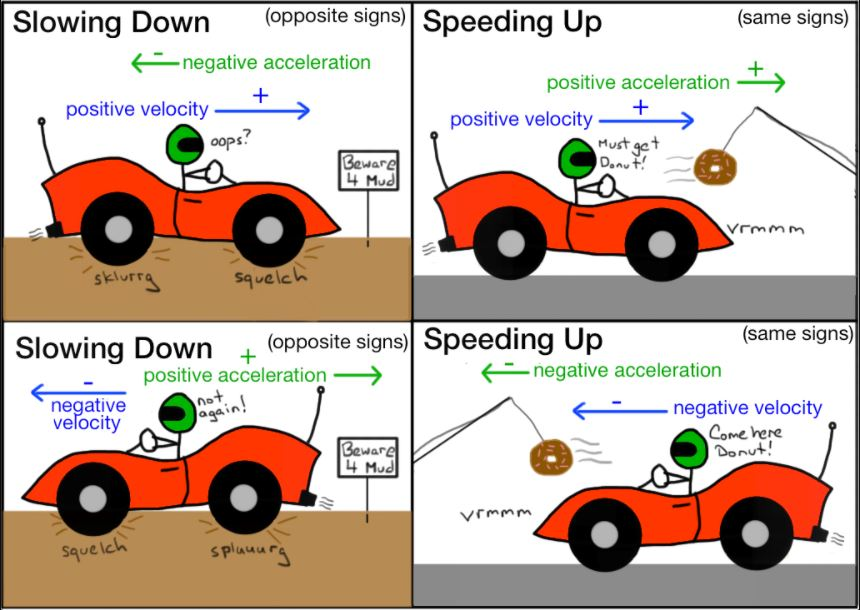
\includegraphics[scale=0.5]{fig4.JPG}}
                    \caption{\href{https://www.khanacademy.org/science/physics/one-dimensional-motion/acceleration-tutorial/a/acceleration-article?modal=1}{source}}
                    \label{fig:posveloaccel}
                \end{center}
            \end{figure}
            \begin{center}
                * * * * *
            \end{center}

            Position, velocity, and acceleration are related in the following way:
            \begin{gather*}
                x'(t) = v(t) \\
                v'(t) = a(t).
            \end{gather*}

        \subsection{Related Rates}
            In simple terms, related rates is using implicit differentiation and given variables to solve for unknown variables. % i feel like more examples should be given in this section. i'm only going to do 2 for now
            \\ Examples:
            \begin{enumerate}
                \item Given the equation: $\frac{x}{y} = 9$ and, $\frac{dy}{dt} = -\frac{2}{3}$, \textbf{find} $\frac{dx}{dt}$ \textbf{when} $x=3$.
                \newline \newline
                \textbf{Solution}:
                \\ First differentiate $\frac{x}{y} = 9$ with respect to $t$.
                \begin{align*}
                    \frac{x}{y} &= 9 \\[6pt]
                    \frac{y \cdot \frac{dx}{dt} - x \cdot \frac{dy}{dt}}{y^2} &= 0
                \end{align*}
                To solve for $\frac{dx}{dt}$, we first have to solve for $y$.
                \begin{align*}
                    \frac{x}{y} &= 9 \\[6pt]
                    \frac{3}{y} &= 9 \\[6pt]
                    y &= \frac{1}{3}
                \end{align*}
                Finally, plugging in all the variables.
                \begin{align*}
                    \frac{y \cdot \frac{dx}{dt} - x \cdot \frac{dy}{dt}}{y^2} &= 0 \\[6pt]
                    \frac{\frac{1}{3} \cdot \frac{dx}{dt} - 3 \cdot -\frac{2}{3}}{\left( \frac{1}{3} \right)^2} &= 0 \\[6pt]
                    \frac{\frac{dx}{dt} }{3} + 2 &= 0 \\[6pt]
                    \frac{\frac{dx}{dt}}{3} &= -2 \\[6pt]
                    \frac{dx}{dt} &= -6
                \end{align*}

                \item The surface area of a sphere is increasing at a rate of $14 \pi$ square meters per hour. At a certain instant, the surface area is $26 \pi$ square meters.
                \\ \textbf{What is the rate of change of the volume of the sphere at that instant (in cubic meters per hour)?}
                \\ (Question from Khan Academy)
                \newline \newline
                \textbf{Solution:}
                \\ The surface area ($SA$) of a sphere with radius $r$ is $4 \pi r^2$.
                \\ The volume ($V$) of a sphere with radius $r$ is $\frac{4}{3} \pi r^3$.
                \\ First identify what is given:
                \begin{itemize}
                    \item $SA = 36 \pi$
                    \item $\frac{dSA}{dt} = 14 \pi$
                \end{itemize}
                Next, what is unknown:
                \begin{itemize}
                    \item $r$, the radius of the sphere.
                    \item $\frac{dr}{dt}$, the rate of change of the radius at the instant specified.
                    \item $V$, the volume of the sphere (it will be seen later that this is actually not needed, $36 \pi$ if you're curious).
                    \item $\frac{dV}{dt}$, the rate of change of the volume at the instant specified (what the question is asking for).
                \end{itemize}
                Solving for $r$:
                \begin{align*}
                    SA &= 4 \pi r^2 \\
                    36 \pi &= 4 \pi r^2 \\
                    9 &= r^2 \\
                    r &= 3
                \end{align*}
                Next, take the derivative of $SA = 4 \pi r^2$ with respect to time, $t$, to solve for the rate of change of $r$ at the instant.
                \begin{align*}
                    SA &= 4 \pi r^2 \\
                    \frac{dSA}{dt} &= 8 \pi r \frac{dr}{dt} \\[6pt]
                    14 \pi &= 24 \pi \frac{dr}{dt} \\[6pt]
                    \frac{dr}{dt} &= \frac{7}{12}
                \end{align*}
                Finally, take the derivative of $V = \frac{4}{3} \pi r^3$ with respect to time, $t$, to solve for the rate of change of volume.
                \begin{align*}
                    V &= \frac{4}{3} \pi r^3 \\[6pt]
                    \frac{dV}{dt} &= \frac{4}{3} \pi 3r^2 \frac{dr}{dt} \\[6pt]
                    &= 4 \pi r^2 \frac{dr}{dt} \quad \text{\hyperlink{relratessphere}{*}}\\[6pt]
                    &= 4 \pi 3^2 \cdot \frac{7}{12} \\[6pt]
                    \frac{dV}{dt} &= 21 \pi
                \end{align*}
                \hypertarget{relratessphere}{*}Note that $4 \pi r^2$ also happens to be the surface area of the sphere.
            \end{enumerate}

        \subsection{Local Linearity and Approximation}
            \textbf{Local linearity} is the understanding that if we zoom in really, really close to a point on a graph that is differentiable on all points in its domain, it would eventually be a straight line, \textit{the tangent line}.
            \\ The general formula for the equation of the tangent line of function $u$ at $x=a$ is:
            \[ y=u'(a)(x-a) + u(a). \]
            \\ This can be useful in approximating values on a graph that are close to another, known value. For example, in \hyperref[fig:locallinapprox]{Figure 5}, point A is at $\sqrt{0.25} = 0.5$. Point B is at $\sqrt{0.3}$, which is a bit harder to calculate. But it can be observed that the tangent line at $x=0.25$ comes really close in $y$ value to point B. If the equation of the tangent line was calculated, we could approximate point B.
            \newline \newline
            \textbf{Approximating point B in \hyperref[fig:locallinapprox]{Figure 5}}:
            \\ Point A is at $(0.25, 0.5)$. The slope of the tangent line can be found using differentiation.
            \begin{align*}
                f(x) &= \sqrt{x} \\
                &= x^{\frac{1}{2}} \\
                f'(x) &= \frac{1}{2\sqrt{x}}
            \end{align*}
            Plugging in all of this into the line equation:
            \begin{align*}
                y &= f'(0.25)(x-0.25) + f(0.25) \\
                &= 1(x-0.25) + 0.5 \\
                y &= x+0.25
            \end{align*}
            Now plugging in the $x$ value of point B, which is $0.3$:
            \begin{align*}
                y &= 0.3 + 0.25 \\
                y &= 0.55
            \end{align*}
            The approximation for point B is $(0.3, 0.55)$. Using a calculator, the real value of B is $(0.3, 0.5477)$, which is really close.
            \begin{figure}[h]
                \begin{center}
                    \frame{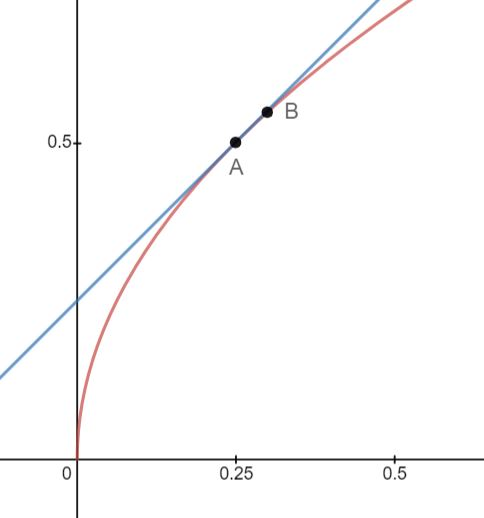
\includegraphics[scale=0.5]{fig5.JPG}}
                    \caption{the red (curved) line is $\sqrt{x}$, with its blue tangent line at $x=0.25$.}
                    \label{fig:locallinapprox}
                \end{center}
            \end{figure}
            \\ Another example of this, in a more similar formatting to what would be on an AP exam:
            \\ Let $g$ be a differentiable function with $g(4) = 6$ and $g'(4) = -2$.
            \\ \textbf{What is the value of the approximation of $g(4.2)$ using the function's local linear approximation at $x=4$?}
            \newline \newline
            \centerline{Plug all of the given information into the line equation formula.}
            \begin{align*}
                y &= g'(4)(x-4) + g(4) \\
                &= -2(x-4) + 6 \\
                &= -2x + 8 + 6 \\
                y &= -2x + 14
            \end{align*}
            \centerline{Now solve with $x=4.2$:}
            \begin{align*}
                y &= -2 \cdot 4.2 + 14 \\
                &= -8.4 + 14 \\
                y &= 5.6
            \end{align*}

        \subsection{L'Hôpital's Rule} % some spellings say l'hospital
            L'Hôpital's Rule states the following:
            \begin{gather*}
                \text{IF} \\
                \lim_{x \to c} \frac{f(x)}{g(x)} = \frac{0}{0} \quad \text{OR} \quad \lim_{x \to c} \frac{f(x)}{g(x)} = \frac{\pm \infty}{\pm \infty} \\[6pt]
                \text{THEN} \\
                \lim_{x \to c} \frac{f(x)}{g(x)} = \lim_{x \to c} \frac{f'(x)}{g'(x)}
            \end{gather*}
            Examples:
            \begin{enumerate}
                \item Indeterminate form $\frac{0}{0}$:
                \begin{gather*}
                    \lim_{x \to 0} \frac{\sin{x}}{x} = \frac{0}{0} \\[6pt]
                    \text{Take the derivative of the top and bottom (separately).}\\
                    \text{According to L'Hopital's rule:} \\
                    \lim_{x \to 0} \frac{\sin{x}}{x} = \lim_{x \to 0} \frac{\cos{x}}{1} \\[6pt]
                    = \frac{1}{1} \\[6pt]
                    = 1
                \end{gather*}
                \item Indeterminate form $\frac{\infty}{\infty}$: $\lim_{x \to \infty} \frac{e^x}{x^2}$
                \begin{gather*}
                    \lim_{x \to \infty} \frac{e^x}{x^2} = \frac{\infty}{\infty} \\[6pt]
                    \text{Take the derivative of the top and bottom (separately).}\\
                    \text{According to L'Hopital's rule:} \\
                    \lim_{x \to \infty} \frac{e^x}{x^2} = \lim_{x \to \infty} \frac{e^x}{2x} \\[6pt]
                    \lim_{x \to \infty} \frac{e^x}{2x} = \frac{\infty}{\infty} \\[6pt]
                    \text{Apply L'Hopital's rule again:} \\
                    \lim_{x \to \infty} \frac{e^x}{2x} = \lim_{x \to \infty} \frac{e^x}{2} \\[6pt]
                    = \frac{\infty}{2} \\[6pt]
                    = \infty
                \end{gather*}
            \end{enumerate}

    \section{Analytical Applications of Differentiation}
    \par\noindent\rule{\textwidth}{0.1pt}
        %* intro here?
        \subsection{Mean Value Theorem}
            \begin{wrapfigure}[11]{r}{0.5\textwidth}
                \begin{center}
                    \frame{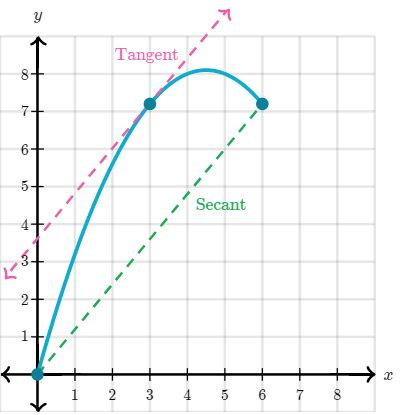
\includegraphics[scale=0.6]{fig6.JPG}}
                \end{center}
                \caption{\href{https://www.khanacademy.org/math/ap-calculus-bc/bc-diff-analytical-applications-new/bc-5-1/a/mean-value-theorem-review?modal=1}{source}}
                \label{fig:meanvaluetheorem}
            \end{wrapfigure}
            The mean value theorem states that for any arc between two endpoints on a graph, there will be a point whose tangent line will be parallel to the secant line between the two endpoints.
            \\ More precisely, given a \textbf{continuous and differentiable} function $f$, in the interval $[a, b]$, there exists a number $c$ such that $f'(c)$ is equal to the average rate of change over $[a, b]$.
            \newline
            \begin{equation*}
                \hspace*{-85mm}
                f'(c) = \frac{f(b)-f(a)}{b-a}
            \end{equation*}
            \newline
            \textit{See \hyperref[fig:meanvaluetheorem]{Figure 6}.}

        \subsection{Extreme Value Theorem}
            If $f(x)$ is a continuous function over the closed interval $[a, b]$, then there exists a maximum and minimum value of $f(x)$.
            \\ More formally, there must exist numbers $c$ and $d$ in $[a, b]$ such that:
            \[ f(c) \le f(x) \le f(d) \quad \forall x \in [a, b] \]
            ($\forall$ means for all.)

        \subsection{First Derivative Test, Second Derivative Test, and Candidates Test}
            The first derivative test, second derivative test, and candidates test are used together to find relative (local) and absolute (global) extremum in a function.
            \subsubsection{Relative (Local) Extrema}
                A \textbf{relative maximum} is a point where the value of the function is largest. The direction changes from increasing to decreasing (highest point).
                \newline \newline
                Similarly, a \textbf{relative minimum} is a point where the value of the function is smallest. The direction changes from decreasing to increasing (lowest point).
                \newline \newline
                \textbf{Using the first derivative test:}
                \newline
                Critical points are points where the derivative of the function is $0$ or undefined. At critical points, there is either an extrema or a point of inflection. For now, we are only concerned with extrema.
                \\ \textbf{Example:} finding the relative extremum of $f(x) = \frac{x^2}{x-1}$.
                \begin{align*}
                    f(x) &= \frac{x^2}{x-1} \\[6pt]
                    f'(x) &= \frac{x^2-2x}{(x-1)^2}
                \end{align*}
                Find the points where $f'(x)$ is $0$ or undefined:
                \begin{center}
                    \begin{tabular}{|c|c|}
                        \hline
                        $x$ & $f'(x)$ \\
                        \hline \hline
                        $0, 2$ & $0$ \\
                        \hline
                        $1$ & undef \\
                        \hline
                    \end{tabular}
                \end{center}
                Next, test the intervals between the critical points to see whether the function is increasing or decreasing. Simply pick a random number in the interval and see if the derivative is positive or negative at that number.
                \begin{center}
                    \begin{tabular}{|c|c|c|}
                        \hline
                        Interval & $f'(x)$ & Slope of $f(x)$ \\
                        \hline \hline
                        $(-\infty, 0)$ & $+$ & $\nearrow$ \\
                        \hline
                        $(0, 1)$ & $-$ & $\searrow$ \\
                        \hline
                        $(1, 2)$ & $-$ & $\searrow$ \\
                        \hline
                        $(2, \infty)$ & $+$ & $\nearrow$ \\
                        \hline
                    \end{tabular}
                \end{center}
                At $x=0$, $f'(x)$ switches from positive to negative, so $f(x)$ has a relative maximum. Similarly, at $x=2$, $f'(x)$ switches from negative to positive, so $f(x)$ has a relative minimum.

                \textbf{Using the second derivative test:}
                \newline
                The second derivative test can make it a lot easier to determine if a critical point is a maximum or minimum.
                \\ Given
                \[ f'(x) = 0, \]
                then:
                \[ f''(x) \begin{cases}
                    >0 \; \Rightarrow \; \text{Minimum point at $x$} \\
                    <0 \; \Rightarrow \; \text{Maximum point at $x$} \\
                    =0 \; \Rightarrow \; \text{Test is inconclusive}
                \end{cases} \]
                \newline
                One way to remember this is that when $f$ reaches a maximum point, its slope gradually decreases, before reaching $0$ then becoming negative. The slope of the first derivative is the second derivative, so if $f'(x)$ is decreasing, $f''(x)$ is negative. Vice versa for a minimum point.

            \subsubsection{Absolute (Global) Extrema}
                An absolute extrema is a point on a function where it achieves its greatest or least possible value. Finding the absolute extrema is very similar to finding the relative extrema. The only extra thing to consider are the endpoints of the given interval. (Interval can be entire domain.)
                \newline \newline
                \textbf{Example (closed domain):} find the global extrema of $f(x) = x^3+2x^2$ over the interval $-2 \le x \le 1$ (\hyperref[fig:absextremaclosed]{Figure 7}).
                \\ Using the first derivative test to find critical points:
                \begin{gather*}
                    f(x) = x^3 + 2x^2 \\
                    f'(x) = 3x^2 + 4x
                \end{gather*}
                Find the points where $f'(x)$ is $0$ or undefined:
                \begin{center}
                    \begin{tabular}{|c|c|}
                        \hline
                        $x$ & $f'(x)$ \\
                        \hline \hline
                        $-\frac{4}{3}, 0$ & $0$ \\
                        \hline
                    \end{tabular}
                \end{center}
                Next, test the intervals between the endpoints and critical points to see whether they are increasing or decreasing.
                \begin{center}
                    \begin{tabular}{|c|c|c|}
                        \hline
                        Interval & $f'(x)$ & Slope of $f(x)$ \\
                        \hline \hline
                        $(-2, -\frac{4}{3})$ & $+$ & $\nearrow$ \\
                        \hline
                        $(-\frac{4}{3}, 0)$ & $-$ & $\searrow$ \\
                        \hline
                        $(0, 1)$ & $+$ & $\nearrow$ \\
                        \hline
                    \end{tabular}
                \end{center}
                Over the closed interval, $(-2, 0)$ and $(0, 0)$ are the relative minimums and $(-\frac{4}{3}, 1.185)$ and $(1, 3)$ are the relative maximums.
                \newline \newline
                \textbf{Both $(-2, 0)$ and $(0, 0)$ have the same $y$ value, so they are both absolute minimums. $(1, 3)$ has the greatest $y$ value so it's the absolute maximum.}
                \begin{figure}[h]
                    \begin{center}
                        \frame{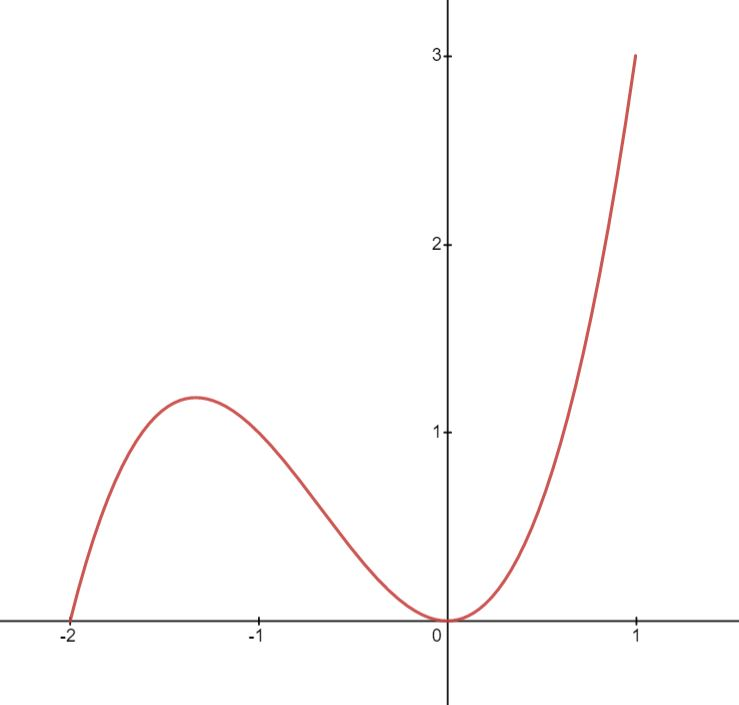
\includegraphics[scale=0.5]{fig7.JPG}}
                        \caption{$f(x) = x^3 + 2x^2 \; \{-2 \le x \le 1 \}$}
                        \label{fig:absextremaclosed}
                    \end{center}
                \end{figure}

            \subsubsection{Concavity and Points of Inflection}
                \begin{wrapfigure}{r}{0.5\textwidth}
                    \begin{center}
                        \frame{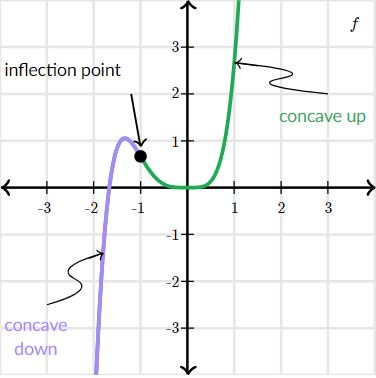
\includegraphics[scale=0.8]{fig8.JPG}}
                    \end{center}
                    \caption{\href{https://www.khanacademy.org/math/ap-calculus-ab/ab-diff-analytical-applications-new/ab-5-6b/a/review-analyzing-the-second-derivative-to-find-inflection-points}{source}}
                    \label{fig:concavityinflection}
                \end{wrapfigure}

                Concavity is the sign of curvature of a function. Parts of a graph can either be \textit{concave up} or \textit{concave down}. When the concavity is concave up, the first derivative is increasing, thus the second derivative is positive. When the concavity is concave down, the first derivative is decreasing, thus the second derivative is negative.
                \\ Inflection points are where the concavity flips. At inflection points both the first and second derivatives are $0$.
                \\ \textbf{Note: when checking if a candidate is an inflection point, the second derivative must change signs!}

        \subsection{Sketching Graphs and Derivatives of Functions} %this is on the college board website, don't know how relevant this is, needs more work
            Find maximums, minimums, and points of inflection using first and second derivative tests. It may also be useful to find the zeroes of the function. Then just connect the dots to make the graph.

        \subsection{Solving Optimization Problems}
            Optimization problems involve finding the largest or smallest something can be. This can be done by first finding a $f(x)$ to represent the relationship, then using $f'(x)$ to find the maximum or minimum.
            \\ \textbf{Examples:}
            \begin{enumerate}
                \item Find the $x$ value for which $y=2x+3$ is the closest to the origin.
                \newline \newline
                \textbf{Solution:}
                    \\ Distance from $(x, y)$ to the origin is:
                    \[ D = \sqrt{x^2 + y^2}. \]
                    Plug in the given equation:
                    \begin{align*}
                        D &= \sqrt{x^2 + y^2} \\
                        D(x) &= \sqrt{x^2 + (2x+3)^2} \\
                        &= \sqrt{5x^2 + 12x + 9}.
                    \end{align*}
                    Next, take the derivative of $D(x)$ to find its minimum. It may actually be hard to solve for the $0$s or undefined values of $D'(x)$, so let $L(x) = \left( D(x) \right )^2$. These two functions will have their minimum values at the same $x$, so just take the derivative of $L(x)$ instead.
                    \begin{align*}
                        L(x) &= 5x^2 + 12x + 9 \\
                        L'(x) &= 10x + 12
                    \end{align*}
                    Find its critical points where it is $0$ or undefined.
                    \begin{align*}
                        L'(x) &= 0 \\
                        10x + 12 &= 0 \\
                        x &= -\frac{6}{5}
                    \end{align*}
                    Use the second derivative test to see if $x=-\frac{6}{5}$ is actually a minimum value.
                    \begin{align*}
                        L'(x) &= 10x + 12 \\
                        L''(x) &= 10
                    \end{align*}
                    Because $L''(x)$ is always positive for all $x$, it can be concluded that $x=-\frac{6}{5}$ is indeed a minimum point, and the final answer.
                    \begin{center}
                        * * * * *
                    \end{center}
                \item Find the maximum product of two positive numbers whose sum is $300$.
                \newline \newline
                    \textbf{Solution:}
                    \\ The question asks to maximize $xy$ given $x+y=300$. The first step is to represent this in a function in terms of $x$, $f(x)$.
                    \begin{align*}
                        x+y &= 300 \\
                        y &= 300 - x \\
                        xy &= x(300-x) \\
                        f(x) &= x(300-x) \\
                        &= 300x - x^2
                    \end{align*}
                    Following the same steps as the previous example to find the maximum of $f(x)$:
                    \begin{align*}
                        f(x) &= 300x - x^2 \\
                        f'(x) &= 300 - 2x.
                    \end{align*}
                    Find critical points:
                    \begin{align*}
                        f'(x) &= 0 \quad \text{(or undefined)} \\
                        300 - 2x & = 0 \\
                        x &= 150.
                    \end{align*}
                    Second derivative test:
                    \begin{align*}
                        f'(x) &= 300 - 2x \\
                        f''(x) &= -2 \\
                        f''(x) &< 0 \quad \forall \; x \in \mathbb{R}
                    \end{align*}
                    Therefore, the $x$ value that yields the maximum product is $150$. Now to find $y$:
                    \begin{align*}
                        x + y &= 300 \\
                        150 + y &= 300 \\
                        y &= 150
                    \end{align*}
                    \[ \therefore x=150, \; y=150. \]
                    \begin{center}
                        * * * * *
                    \end{center}

                \item We want to construct a cylindrical can with a bottom but no top that will have a volume of $30$ cm\textsuperscript{3}. Determine the dimensions of the can that will minimize the amount of material needed to construct the can.
                \newline \newline
                    \textbf{Solution:}
                    \begin{gather*}
                        V = \pi r^2 h \\
                        SA = \pi r^2 + 2\pi rh
                    \end{gather*}
                    Solve for $h$ to minimize $r$:
                    \begin{align*}
                        \pi r^2 h &= 30 \\
                        h &= \frac{30}{\pi r^2}.
                    \end{align*}
                    Plug this into the $SA$ equation:
                    \begin{align*}
                        SA(r) &= \pi r^2 + 2\pi r \left( \frac{30}{\pi r^2} \right) \\[6pt]
                        &= \pi r^2 + \frac{60}{r}
                    \end{align*}
                    Take derivative and find the critical points:
                    \begin{gather*}
                        SA'(r) = 2 \pi r - \frac{60}{r^2}. \\[6pt]
                        \text{Critical points at:} \\
                        r = 0, \; \sqrt[3]{\frac{30}{\pi}} \\[6pt]
                        \text{*Note that $r=0$ does not exist, as the radius can not be $0$.}
                    \end{gather*}
                    Second derivative test:
                    \begin{gather*}
                        SA''(r) = 2 \pi + \frac{120}{r^3} \\[6pt]
                        SA'' \left( \sqrt[3]{\frac{30}{\pi}} \right) > 0 \\[6pt]
                        \therefore \sqrt[3]{\frac{30}{\pi}} \; \text{is the minimum} \; r.
                    \end{gather*}
                    Plug $r$ into $h=\frac{30}{\pi r^2}$.
                    \\ Final answer:
                    \begin{gather*}
                        r = \sqrt[3]{\frac{30}{\pi}} \\[6pt]
                        h \approx 2.1215.
                    \end{gather*}
            \end{enumerate}

        \subsection{Behaviors of Implicit Relations} % x and y values in original equation and derivative go back and forth? what's a good way to explain this...
            Implicit relations can be useful in solving for unknown values or line equations. The key takeaway is that the variables used in the original function can be substituted back and forth with its higher order derivatives.
            \newline \newline
            \textbf{Examples:}
            \begin{enumerate}
                \item Consider the curve given by $x^3 + xy = -2$. It can be shown that $\frac{dy}{dx} = \frac{-3x^2 - y}{x}$.
                    \\ Find the point where the tangent line of the curve is horizontal.
                    \newline \newline
                    \textbf{Solution:}
                    \\ For the tangent line to be horizontal, the slope has to be $0$. This means that the numerator of $\frac{dy}{dx}$ must be $0$, but the denominator can not be $0$. Simply solve the system of equations:
                    \[ \begin{cases}
                        x^3 + xy = -2 \\
                        -3x^2 - y = 0 \\
                        x \ne 0.
                    \end{cases} \]
                    \begin{align*}
                        -3x^2 - y &= 0 \\
                        y &= -3x^2 \\[6pt]
                        x^3 + x(-3x^2) &= -2 \\
                        x^3 - 3x^3 &= -2 \\
                        -2x^3 &= -2 \\
                        x &= 1 \\[6pt]
                        y &= -3(1)^2 \\
                        &= -3
                    \end{align*}
                    Therefore, at $(1, -3)$, the slope of the tangent line is $0$, and thus it is horizontal.
            \end{enumerate}

    \section{Integration and Accumulation of Change (17\% - 20\%)}
    \par\noindent\rule{\textwidth}{0.1pt}
        The accumulation of change is the net change of a quantity. This is not the same thing as simply the quantity. The accumulation of change takes into consideration time, and it is the quantity over a specified time period. There may be some quantity before or after this time period, but we would not count that.

        \subsection{Riemann Sums}
            A Riemann Sum approximates the area under a curve by splitting it up into rectangles.

            \subsubsection{Types of Riemann Sums}
                \begin{itemize}
                    \item \textbf{Left Riemann Sums} line up the left side of the rectangle with the curve of the function.
                    \begin{figure}[H]
                        \begin{center}
                            \frame{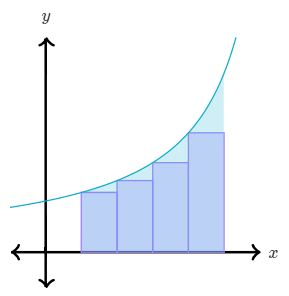
\includegraphics[scale=0.7]{fig9.JPG}}
                            \caption{left Riemann sums, \href{https://www.khanacademy.org/math/ap-calculus-bc/bc-integration-new/bc-6-2/a/riemann-sums-review?modal=1}{source}}
                        \end{center}
                    \end{figure}
                    \item \textbf{Right Riemann Sums} line up the right side of the rectangle with the curve of the function.
                    \begin{figure}[H]
                        \begin{center}
                            \frame{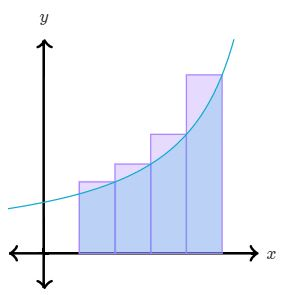
\includegraphics[scale=0.7]{fig10.JPG}}
                            \caption{right Riemann sums, \href{https://www.khanacademy.org/math/ap-calculus-bc/bc-integration-new/bc-6-2/a/riemann-sums-review?modal=1}{source}}
                        \end{center}
                    \end{figure}
                    \item \textbf{Midpoint Riemann Sums} line up the middle of the rectangle with the curve of the function.
                    \begin{figure}[H]
                        \begin{center}
                            \frame{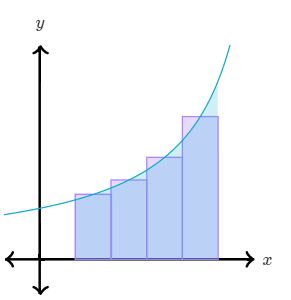
\includegraphics[scale=0.7]{fig11.JPG}}
                            \caption{midpoint Riemann sums, \href{https://www.khanacademy.org/math/ap-calculus-bc/bc-integration-new/bc-6-2/a/riemann-sums-review?modal=1}{source}}
                        \end{center}
                    \end{figure}
                    \item There is another way to approximate areas under a curve, called a \textbf{trapezoidal sum}. Trapezoids are used, and its two bases touch the curve of the function.
                    \begin{figure}[H]
                        \begin{center}
                            \frame{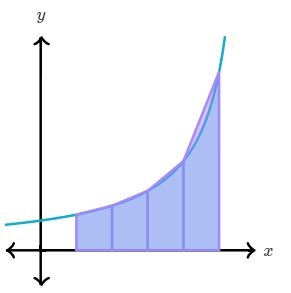
\includegraphics[scale=0.7]{fig12.JPG}}
                            \caption{trapezoidal sums, \href{https://www.khanacademy.org/math/ap-calculus-bc/bc-integration-new/bc-6-2/a/riemann-sums-review?modal=1}{source}}
                        \end{center}
                    \end{figure}
                \end{itemize}
                With each type of sum, the more shapes that we have, the closer the approximation would be to the actual area. This can be achieved by making $\Delta x$, the base of the rectangle, smaller and smaller.

            \subsubsection{Riemann Sums in Summation Notation}
                Given a Riemann sum over the interval $[a, b]$ with $n$ rectangles of equal width, we can define $\Delta x = \frac{b-a}{n}$. The bottom right corner of each rectangle will be $x_i$, so $x_i = a + \Delta x \cdot i$.
                \begin{center}
                    \begin{tabular}{|c|c|}
                        \hline
                        Left & Right \\
                        \hline \hline
                        $\displaystyle \sum_{i=0}^{n-1} \Delta x \cdot f(x_i)$ & $\displaystyle \sum_{i=1}^{n} \Delta x \cdot f(x_i)$ \\
                        \hline
                    \end{tabular}
                \end{center}

        \subsection{Definite Integrals} %* where to include solving definite integrals?
            As $\Delta x$ gets smaller and smaller in Riemann Sums, we are able to get better and better approximations of the area under a curve. However, it is impossible to calculate the exact area under the curve using a finite number of rectangles. In order to do so, we need an infinitely small $\Delta x$, or a limit that approaches $0$.
            \\ Indefinite integrals can find the \textit{exact} area of an interval under a curve.
            \newline \newline
            The definite integral notation over the interval $[a, b]$ of $f(x)$ is:
            \[ \int_{a}^{b} f(x) \, dx. \]
            The connection between a definite integral and Riemann sum is as follows:
            \[ \int_{a}^{b} f(x) \, dx = \lim_{n \to \infty} \sum_{i=1}^{n} \Delta x \cdot f(x_i) \]
            where $\Delta x = \frac{b-a}{n}$ and $x_i = a + \Delta x \cdot i$.
            \begin{center}
                * * * * *
            \end{center}
            \textbf{Example of writing definite integral as Riemann sum:}
            \[ \int_{\pi}^{2 \pi} \sin{(x)} \, dx \]
            First find $\Delta x$:
            \begin{align*}
                \Delta x &= \frac{b-a}{n} \\[6pt]
                &= \frac{2 \pi - \pi}{n} \\[6pt]
                &= \frac{\pi}{n}.
            \end{align*}
            Next, find $x_i$:
            \begin{align*}
                x_i &= a + \Delta x \cdot i \\
                &= \pi + \frac{\pi}{n} \cdot i \\[6pt]
                &= \pi + \frac{\pi i}{n}.
            \end{align*}
            Putting everything together:
            \begin{align*}
                \int_{a}^{b} f(x) \, dx &= \lim_{n \to \infty} \sum_{i=1}^{n} \Delta x \cdot f(x_i) \\[6pt]
                \int_{\pi}^{2 \pi} \sin{(x)} \, dx &= \lim_{n \to \infty} \sum_{i=1}^{n} \frac{\pi}{n} \cdot \cos{\left( \pi + \frac{\pi i}{n} \right)}.
            \end{align*}

        \subsection{The Fundamental Theorem of Calculus}
            The fundamental theorem of calculus goes as follows:
            \newline \newline
            Let $f$ be a function that is continuous over the interval $[a, b]$, and let:
            \[ F(x) = \int_{a}^{x} f(t) \, dt. \]
            $F$ is the antiderivative of $f$, or in other words, the derivative of $F$ is $f$. This can then tell us how to solve for the area under a curve using antidifferentiation.
            \[ \int_{a}^{b} f(x) \, dx = F(b) - F(a) \]

        \subsection{Antiderivatives}
            Antiderivatives are how to get from $f'(x)$ back to $f(x)$.
            \subsubsection{Basic Rules}

            \subsubsection{Substitution}

        \subsection{Solving Definite Integrals}

        \subsection{Solving Indefinite Integrals}


        \subsection{Integration Techniques}

        \subsection{Improper Integrals}

    \section{Differential Equations (6\% - 9\%)}

    \section{Applications of Integration (6\% - 9\%)}

    \section{Parametric Equations, Polar Coordinates, and Vector-Valued Functions (11\% - 12\%)}

    \section{Infinite Sequences and Series (17\% - 18\%)}
\end{document}
